\section{SENTRY-R: scenario-enriched neural triage for release review}\label{sec:sentry}

We name the implementable extension \emph{SENTRY-R}, shorthand for
scenario-enriched neural triage for release review. This names the specified
workflow, not a claim that its
components are individually new or that a fitted network has improved real
release decisions. Its separation of three data streams is central:
\emph{untrusted scenario proposals}, \emph{measured development attacks}, and
\emph{untouched final audits}. The implementation supports any finite input
dimension $d$ and any finite number $n$ of declared risk coordinates. A deeper
network predicts attack frequencies for search; it does not certify a release.

\subsection{LLM-assisted scenario expansion and evidence provenance}

Let $\mathcal F_t$ denote the information available before development round
$t$, including past mechanisms, validated scenario specifications and measured
attacks. A language model proposes descriptions and numeric scenario features
$Q_t=G_t(\mathcal F_t,\xi_t)$. A deterministic validator checks the predeclared
feature names and bounds and the scenario identifier. The calling code, not
the language model, writes the source metadata: the model name and the
SHA-256 hash of the exact prompt. The validator does
not treat free-form text or a language-model risk estimate as an observed
success. A separate attack evaluator then draws $Z_{ti}$ under the accepted
scenario and records $K_{tj}=\sum_{i=1}^{B_{tj}}s_j(Z_{ti})$, together with
its experiment identifier and sampling unit. The retraining history grows by
\begin{equation}
 \mathcal F_{t+1}=\mathcal F_t\vee\sigma\!\left(Q_t,\operatorname{valid}(Q_t),
 \{K_{tj},B_{tj},\operatorname{provenance}_{tj}\}_{j\in\mathcal J}\right).
 \label{eq:sentry-filtration}
\end{equation}
The language model can change which \emph{development} experiment is run next;
it does not directly change a network weight or label. Source identifiers,
scenario hashes and an explicit partition label make the update inspectable.
Treating repeated targets or auxiliary files as independent Bernoulli trials
would break the specified sampling model. Human review is still required to
establish whether a proposed adversary, harm definition and auxiliary source
are plausible and permissible.

Let $\mathcal D=\mathcal F_{t_*}$ be all such development information at a
chosen stopping time $t_*$, including model weights and hyperparameter
selection. A separate validation set holds out entire release programmes;
final audit draws are excluded from $\mathcal D$. Conditional on $\mathcal D$,
freeze the coordinate definitions, policy tolerances, $C$ shortlisted
candidates, the family error $\alpha$ and the planned sample sizes
$B_{\theta j}$. The implementation writes all of these, with a named
tolerance owner, an expiry date and every development evidence identifier,
into one hashed freeze record. The final audit reads $\alpha$ from that
record and refuses to run if the record has changed, if the expiry date has
passed, if any trial count differs from the plan, or if an audit evidence
identifier was used in development. An optional append-only ledger refuses a
second audit of the same freeze. These checks bind an audit to its freeze.
On their own they do not prove the order of events, since the freeze hash has
no key or trusted time stamp. An optional keyed ledger records a stronger
local history: each instrumented stage, from the language model's proposal through
review, measurement, training and freeze to the audit, is appended to one
hash-chained file, each entry signed with HMAC-SHA256 under a key the operator
holds, and an entry is refused unless the entries it depends on are already on
the chain. The same ledger holds each programme's error budget and debits
every recorded audit's $\alpha$ against it. New measurement entries also commit
the full measured row, so changed features or counts are refused when recording
a training artifact. These checks apply when provenance and proposal lineage
are retained. Base evidence, reviewer identities and evaluator authenticity
remain caller-controlled, and an operator can omit provenance or relabel data.
The audit debit occurs after outcomes are supplied; it does not prevent an
operator from obtaining or discarding outcomes outside the recorded path. A
service must reserve budget before draws, preserve every attempt and anchor
chain heads outside the operator's control. A key holder can otherwise rewrite
the file. Under the stated statistical assumptions, Proposition
\ref{prop:neural-gate} guarantee then applies even if the \emph{development}
sequence used an LLM adaptively, provided the conditional binomial model for
the untouched final draws holds. A final audit reused as development data, or
an LLM proposal generated from its outcomes, invalidates that conditioning.
Figure \ref{fig:sentry-loop} shows the implemented boundary. It reads from left
to right and then down. A scenario proposed by a language model passes a fixed
schema and a named review, and it can add a scenario but never an outcome. Only
counted development attacks train the deep proposal model, whose ranking fixes a
shortlist of candidate settings. Only the fresh final audit, with simultaneous
bounds over every coordinate, reaches the release decision. The note under the
first box states the rule the figure is there to show: proposal text never
supplies a training label or a release certificate.
\begin{figure}[tbp]
\centering
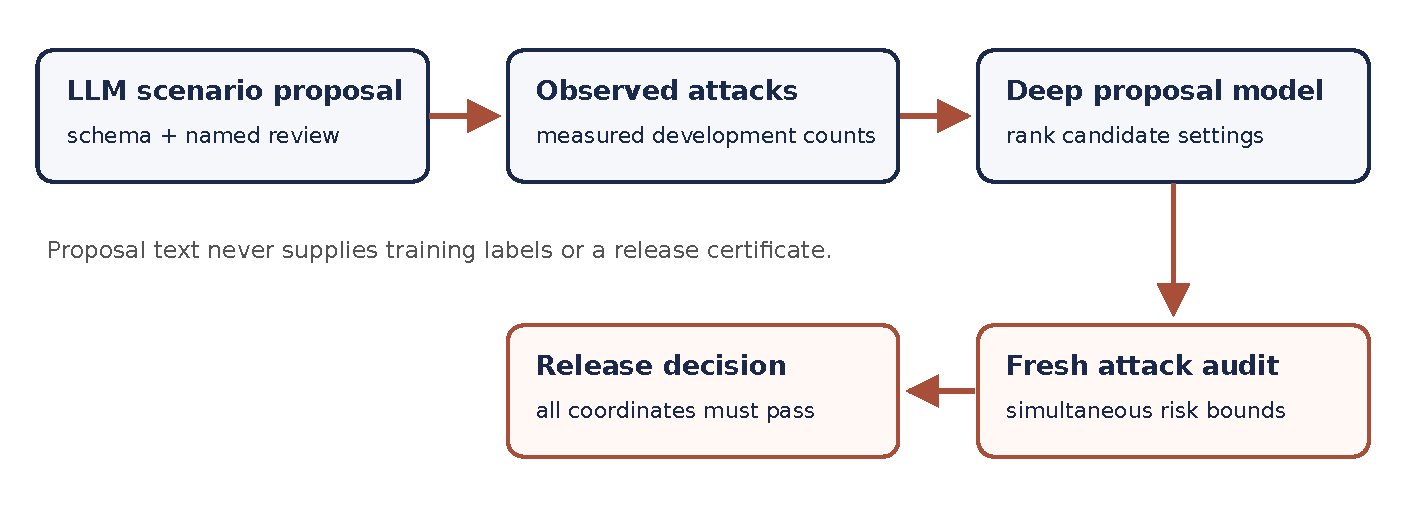
\includegraphics[width=0.95\linewidth]{diagrams/sentry_r_loop.pdf}
\caption{SENTRY-R development and decision boundary. The LLM's scenario proposal is checked against a fixed schema; only measured development attacks enter the deep model. Its ranking freezes a shortlist before a fresh, independent final audit.}
\label{fig:sentry-loop}
\end{figure}


\subsection{A deep model trained on counted attack outcomes}

The \texttt{privacy\_risk.sentry\_r} module provides a depth-$L$ fully connected
ReLU model with common width $q$, including the depth-zero logistic baseline.
Training features $x_i\in\mathbb R^d$ are standardised using \emph{training}
means and scales only. With $h_i^0=x_i$, for $\ell=0,\ldots,L-1$ define
\begin{equation}
 h_i^{\ell+1}=\rho(h_i^\ell W_\ell+b_\ell),\quad
 a_{ij}=\left(h_i^L W_{\mathrm o}+b_{\mathrm o}\right)_j,\quad
 p_{ij}=\sigma(a_{ij}),\quad \rho(z)=\max\{0,z\}.
 \label{eq:sentry-deep}
\end{equation}
For each observed development pair $(i,j)$ let $K_{ij}\in\{0,\ldots,B_{ij}\}$
be the count of successes in $B_{ij}\geq1$ trials. The implementation
minimises the binomial negative log likelihood, without its constant
combinatorial term, and a ridge term:
\begin{equation}
 \mathcal L(\phi)= -\frac{1}{B_\bullet}\sum_{i,j}
 \left[K_{ij}\log p_{ij}+(B_{ij}-K_{ij})\log(1-p_{ij})\right]
 +\frac{\lambda}{2}\sum_{\ell=0}^{L}\|W_\ell\|_F^2,
 \quad B_\bullet=\sum_{i,j}B_{ij}.
 \label{eq:sentry-count-loss}
\end{equation}
Here $W_L=W_{\rm o}$; a weight attached to trial count is appropriate only if
the count's sampling design was fixed without peeking at those outcomes. To
see exactly what is learned, assume $K\mid x,B\sim\mathrm{Binom}(B,\pi_j(x))$
with $B$ determined before outcomes. For a fixed $x,B$, the expected
unregularised loss minus its value at $p=\pi_j(x)$ is
\begin{equation}
 \frac{B}{B_\bullet}\,D_{\mathrm{KL}}
 \left(\mathrm{Bern}(\pi_j(x))\,\|\,\mathrm{Bern}(p)\right)\geq0.
 \label{eq:sentry-proper}
\end{equation}
Thus the ideal unrestricted conditional predictor is the attack success
frequency $\pi_j(x)$ on the \emph{development} distribution; finite data,
regularisation, optimiser error and population shift prevent equality in an
actual trained model. No neural output is a confidence limit on an individual
or a new population.

The model is fitted by backpropagation. With $P=(p_{ij})$, $K=(K_{ij})$ and
$B=(B_{ij})$, the output-logit derivative is $(B\odot P-K)/B_\bullet$, and the
hidden-layer gradients follow by the chain rule in the usual way
\citep[ch.~6]{goodfellow2016}. The package includes a finite-difference check of
the derivatives.

\subsection{Training, scale and falsification}

The network uses seeded mini-batches, Adam, gradient clipping and early
stopping on a separate held-out programme. Depth zero is trained on the same
counted outcomes as a logistic baseline. For $N$ development rows and $E$
epochs, the dense leading arithmetic order is
$O\{EN[dq+(L-1)q^2+qn]\}$ for $L\geq1$, with
$O\{dq+(L-1)q^2+qn\}$ weights; the logistic case has $O(ENdn)$
arithmetic. This is a computational scaling statement, not a statistical
sample-size promise. The final $Cn$ confidence bounds and independent attack
trials remain necessary whatever the prediction speed. Unknown groups and
out-of-domain features trigger a new assessment rather than an extrapolated
certificate.

A valid empirical evaluation must compare deep and logistic rankings at fixed
shortlist sizes and audit budgets on held-out \emph{real} programmes; report
log loss, Brier score, worst-group calibration, selected utility and false
gates; repeat pooled-vintage attacks; and show uncertainty across programmes.
This package currently provides a seeded synthetic end-to-end demonstration,
not such an evaluation. Table \ref{tab:sentry-synthetic} is regenerated by
\texttt{scripts/sentry\_r\_benchmark.py}. For each of ten seeds it draws
three disjoint programmes from one toy law: 320 training rows, 100 rows used
only for early stopping, and 2,000 test rows used only for the reported loss.
Both models train until 150 epochs pass without improvement, and no best
epoch reaches the cap. Trained to convergence, the logistic model has a
slightly lower test log loss than the three-layer model in all ten
replicates. The mean paired gap is smaller than the spread of either model
across replicates. The table shows that the pipeline runs, not that depth
helps. The test programmes come from the same law and feature range as the
training data, so they do not test shift.
\begin{table}[H]
\centering
\small
\caption{Synthetic SENTRY-R comparison over 10 seeded replicates of the toy law. Each replicate draws 320 training rows, 100 rows used only for early stopping (patience 150 epochs, cap 6000) and 2000 test rows used only for the reported losses. Entries are mean (standard deviation) across replicates; smaller is better. The last row is the paired deep-minus-logistic test log loss (range 0.0004 to 0.0050; deep lower in 0 of 10). These are not results on real release programmes.}
\label{tab:sentry-synthetic}
\begin{tabular}{lrrr}
\toprule
Proposal model & Test log loss & Test Brier score & Best epoch (range) \\
\midrule
Logistic & 0.2556 (0.0043) & 0.0727 (0.0017) & 404--898 \\
Three-layer ReLU & 0.2576 (0.0047) & 0.0735 (0.0018) & 79--402 \\
\midrule
Deep minus logistic & 0.0020 (0.0014) & & \\
\bottomrule
\end{tabular}
\end{table}

